\documentclass[10pt]{article}
\usepackage[utf8]{inputenc}
\usepackage[T1]{fontenc}
\usepackage{amsmath}
\usepackage{amsfonts}
\usepackage{amssymb}
\usepackage[version=4]{mhchem}
\usepackage{stmaryrd}
\usepackage{multirow}
\usepackage{graphicx}
\usepackage[export]{adjustbox}
\graphicspath{ {./images/} }

\begin{document}
\begin{center}
\begin{tabular}{|l|l|}
\hline
\multicolumn{2}{|l|}{All answers on this assessment should be simplified and exact. No calculators are allowed.} \\
\hline
\multicolumn{2}{|l|}{Factor each of the following (1 point each)} \\
\hline
1. $x^{2}-8 x+12$ & 2. $6 x^{2}-7 x-3$ \\
\hline
\multicolumn{2}{|c|}{3. Solve the equation shown for $x$ by completing the square. Note that $a$ is a constant and can be in your answer. (5 points)
\(
3 x^{2}-6 a x=4
\)} \\
\hline
 &  \\
\hline
\multicolumn{2}{|l|}{\multirow{2}{*}{\begin{tabular}{l}
4. Solve the equation shown for $x$. (3 points) \( 2 x^{2}+6 x-8=13 x-4 \) \\
Answer: $x=$ $\_\_\_\_$ \\
\end{tabular}}} \\
\hline
 &  \\
\hline
\multicolumn{2}{|c|}{5. If $h(x)=-3 x^{2}+5 b x+2$ has two real roots, give all possible values of $b$. State your answer in interval notation. (3 points)} \\
\hline
\end{tabular}
\end{center}

The function $f(x)$ is a quadratic function with real coefficients and exactly one distinct real root. The graph of $f(x)$ intersects the line $y=\frac{9}{2}$ when $x=1$ and again when $x=5$. Use this information to provide to find the following information about $f(x)$.\\
6. Graph $f(x)$ on the axes below. Be sure to include 3 points on the graph of $f(x)$. (1 point)\\
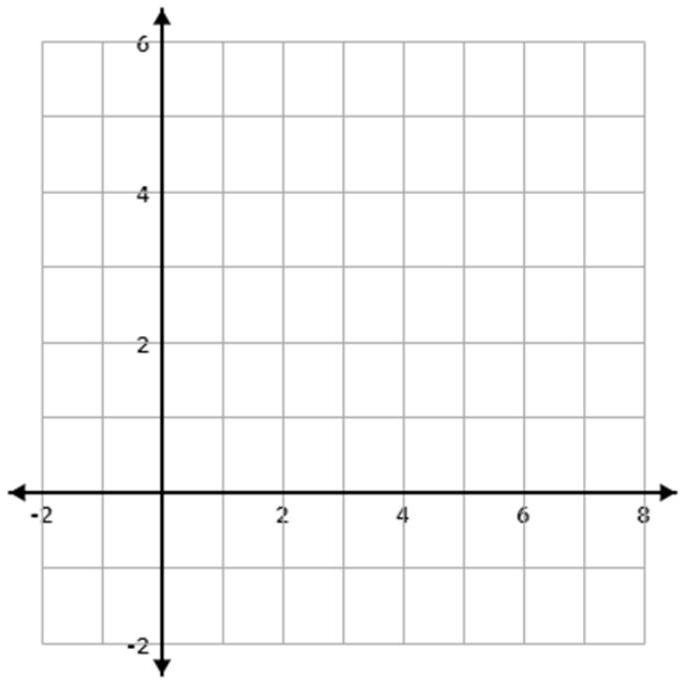
\includegraphics[max width=\textwidth, alt={}, center]{b1ad2e81-5a39-4bac-8cfd-6ebfc7f4a6f6-02_687_687_416_721}\\
7. Write $f(x)$ in vertex form. (2 points)\\
8. Write $f(x)$ in factored form. (1 point)\\
8. Write $f(x)$ in standard form. (1 point)

\begin{center}
\begin{tabular}{|l|}
\hline
All answers on this assessment should be simplified and exact. No calculators are allowed. \\
\hline
Simplify each of the following (1 point each) \\
\hline
9. $\frac{60-14 i}{-4 i+6}$ \\
\hline
11. Solve $4 x^{2}+x+19=x+10$ by factoring. (3 points) \\
\hline
12. A quadratic function $f(x)$ has a root at $\frac{12 i+8}{2 i-3}$ and the graph of $f(x)$ contains the point $(2,40)$. Solve the inequality $f(x) \geq 47-x$. Write your answer in interval notation. (4 points) \\
\hline
\end{tabular}
\end{center}

The graph of a function $f(x)$ is given on the axes below. Use the graph to write $f(x)$ in vertex form, standard form, and factored form.\\
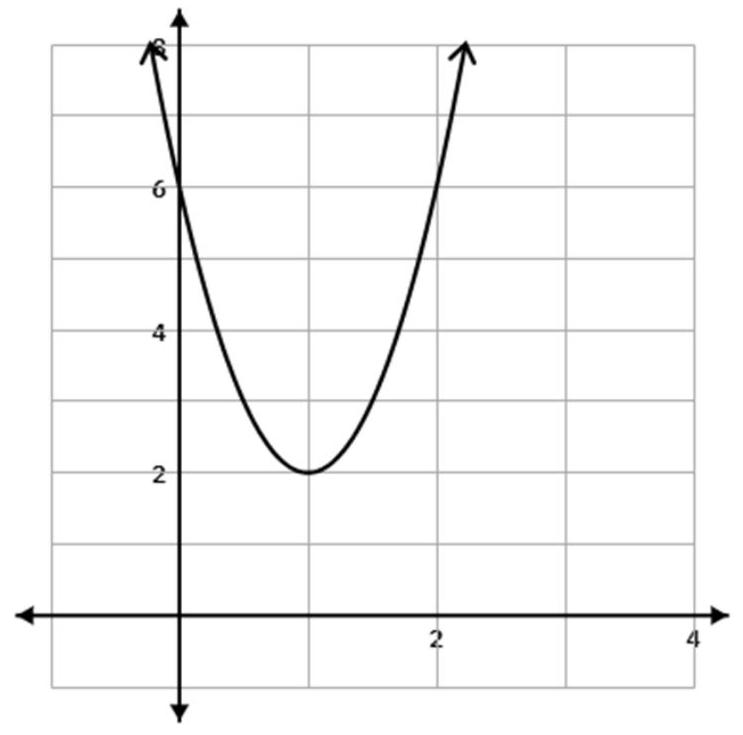
\includegraphics[max width=\textwidth, alt={}, center]{b1ad2e81-5a39-4bac-8cfd-6ebfc7f4a6f6-04_735_743_292_691}\\
13. Write $f(x)$ in vertex form. (2 points)\\
14. Write $f(x)$ in factored form. (1 point)\\
15. Write $f(x)$ in standard form. (1 point)

\begin{center}
\begin{tabular}{|l|l|}
\hline
\multicolumn{2}{|l|}{All answers on this assessment should be simplified and exact. No calculators are allowed.} \\
\hline
\multicolumn{2}{|l|}{Factor each of the following (1 point each)} \\
\hline
1. $x^{2}+7 x+12$ & 2. $9 x^{2}-16 x-4$ \\
\hline
\multicolumn{2}{|c|}{3. Solve the equation shown for $x$ by completing the square. Note that $a$ is a constant and can be in your answer. (5 points)
\(
2 x^{2}-12 a x=2
\)} \\
\hline
 &  \\
\hline
\multicolumn{2}{|l|}{\multirow{2}{*}{\begin{tabular}{l}
4. Solve the equation shown for $x$. (3 points) \( 4 x^{2}+6 x-8=12 x-4 \) \\
Answer: $x=$ $\_\_\_\_$ \\
\end{tabular}}} \\
\hline
 &  \\
\hline
\multicolumn{2}{|c|}{5. If $h(x)=3 x^{2}-2 b x+2$ has two nonreal roots, give all possible values of $b$. State your answer in interval notation. (3 points)} \\
\hline
\end{tabular}
\end{center}

The function $f(x)$ is a quadratic function with real coefficients an exactly one distinct real root. The graph of $f(x)$ intersects the line $y=-1$ when $x=-1$ and again when $x=7$. Use this information to provide to find the following information about $f(x)$.\\
6. Graph $f(x)$ on the axes below. Be sure to include 3 points on the graph of $f(x)$. (1 point)\\
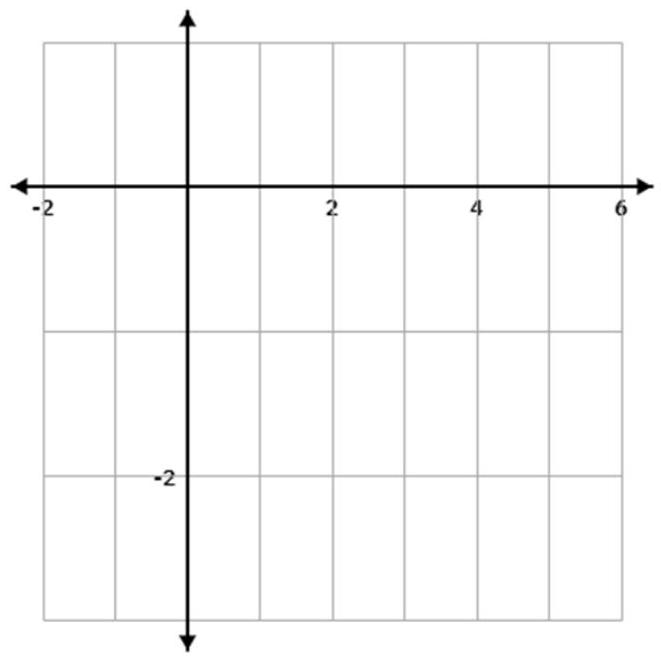
\includegraphics[max width=\textwidth, alt={}, center]{b1ad2e81-5a39-4bac-8cfd-6ebfc7f4a6f6-06_663_661_401_730}\\
7. Write $f(x)$ in vertex form. (2 points)\\
8. Write $f(x)$ in factored form. (1 point)\\
8. Write $f(x)$ in standard form. (1 point)

\begin{center}
\begin{tabular}{|l|}
\hline
All answers on this assessment should be simplified and exact. No calculators are allowed. \\
\hline
Simplify each of the following (1 point each) \\
\hline
9. $\frac{10-4 i}{-2 i+1}$ \\
\hline
11. Solve $16 x^{2}+8 x+19=8 x+10$ by factoring. (3 points) \\
\hline
12. A quadratic function $f(x)$ has a root at $\frac{12 i+6}{2 i-4}$ and the graph of $f(x)$ contains the point $(3,54)$. Solve the inequality $f(x)<5 x+35$. Write your answer in interval notation. (4 points) \\
\hline
\end{tabular}
\end{center}

The graph of a function $f(x)$ is given on the axes below. Use the graph to write $f(x)$ in vertex form, standard form, and factored form.\\
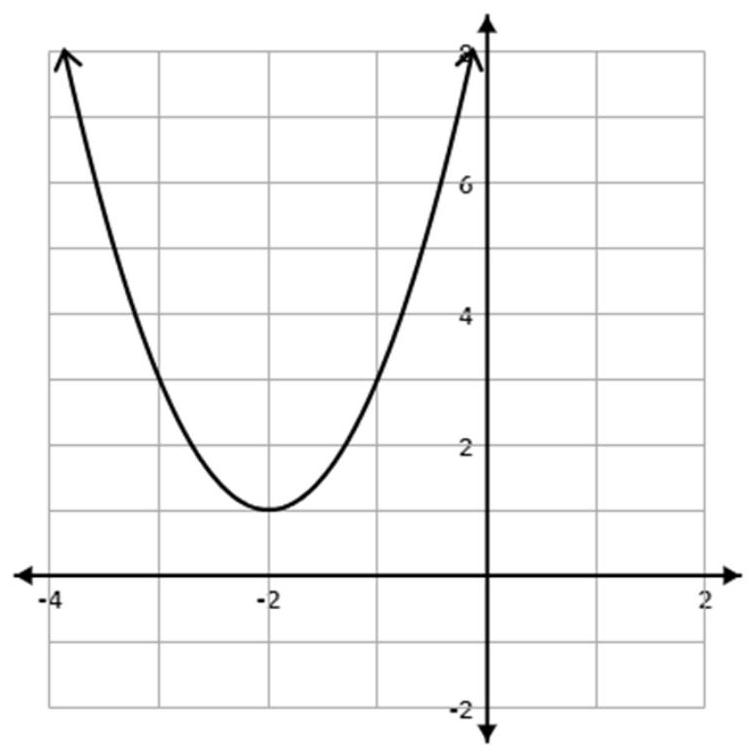
\includegraphics[max width=\textwidth, alt={}, center]{b1ad2e81-5a39-4bac-8cfd-6ebfc7f4a6f6-08_755_753_287_635}\\
13. Write $f(x)$ in vertex form. (2 points)\\
14. Write $f(x)$ in factored form. (1 point)\\
15. Write $f(x)$ in standard form. (1 point)

\begin{center}
\begin{tabular}{|l|l|}
\hline
\multicolumn{2}{|l|}{All answers on this assessment should be simplified and exact. No calculators are allowed.} \\
\hline
\multicolumn{2}{|l|}{Factor each of the following (1 point each)} \\
\hline
1. $x^{2}-12 x-28$ & 2. $3 x^{2}-7 x-6$ \\
\hline
\multicolumn{2}{|c|}{\multirow{2}{*}{\begin{tabular}{l}
3. Solve the equation shown for $x$ by completing the square. Note that $a$ is a constant and can be in your answer. (5 points) \( 2 x^{2}+8 a x=5 \) \\
Answer: $x=$ $\_\_\_\_$ \\
\end{tabular}}} \\
\hline
 &  \\
\hline
\multicolumn{2}{|c|}{\multirow{2}{*}{\begin{tabular}{l}
4. Solve the equation shown for $x$. (3 points) \( 3 x^{2}+6 x-8=13 x-10 \) \\
Answer: $x=$ $\_\_\_\_$ \\
\end{tabular}}} \\
\hline
 &  \\
\hline
\multicolumn{2}{|l|}{5. If $h(x)=-2 x^{2}-7 b x-1$ has two nonreal roots, give all possible values of $b$. State your answer in interval notation. (3 points)} \\
\hline
\end{tabular}
\end{center}

The function $f(x)$ is a quadratic function with real coefficients an exactly one distinct real root. The graph of $f(x)$ intersects the line $y=-4$ when $x=-4$ and again when $x=0$. Use this information to provide to find the following information about $f(x)$.\\
6. Graph $f(x)$ on the axes below. Be sure to include 3 points on the graph of $f(x)$. (1 point)\\
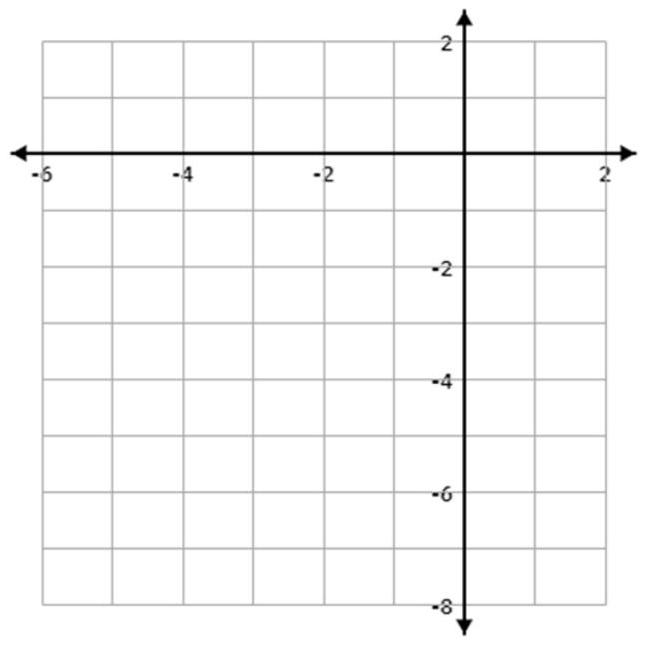
\includegraphics[max width=\textwidth, alt={}, center]{b1ad2e81-5a39-4bac-8cfd-6ebfc7f4a6f6-10_646_646_433_689}\\
7. Write $f(x)$ in vertex form. (2 points)\\
8. Write $f(x)$ in factored form. (1 point)\\
8. Write $f(x)$ in standard form. (1 point)

\begin{center}
\begin{tabular}{|l|}
\hline
All answers on this assessment should be simplified and exact. No calculators are allowed. \\
\hline
Simplify each of the following (1 point each) \\
\hline
9. $\frac{6-4 i}{3 i-5}$ \\
\hline
11. Solve $9 x^{2}+2 x+9=2 x+5$ by factoring. (3 points) \\
\hline
12. A quadratic function $f(x)$ has a root at $\frac{2-10 i}{i+5}$ and the graph of $f(x)$ contains the point $(3,26)$. Solve the inequality $f(x) \leq 12+7 x$. Write your answer in interval notation. (4 points) \\
\hline
\end{tabular}
\end{center}

The graph of a function $f(x)$ is given on the axes below. Use the graph to write $f(x)$ in vertex form, standard form, and factored form.\\
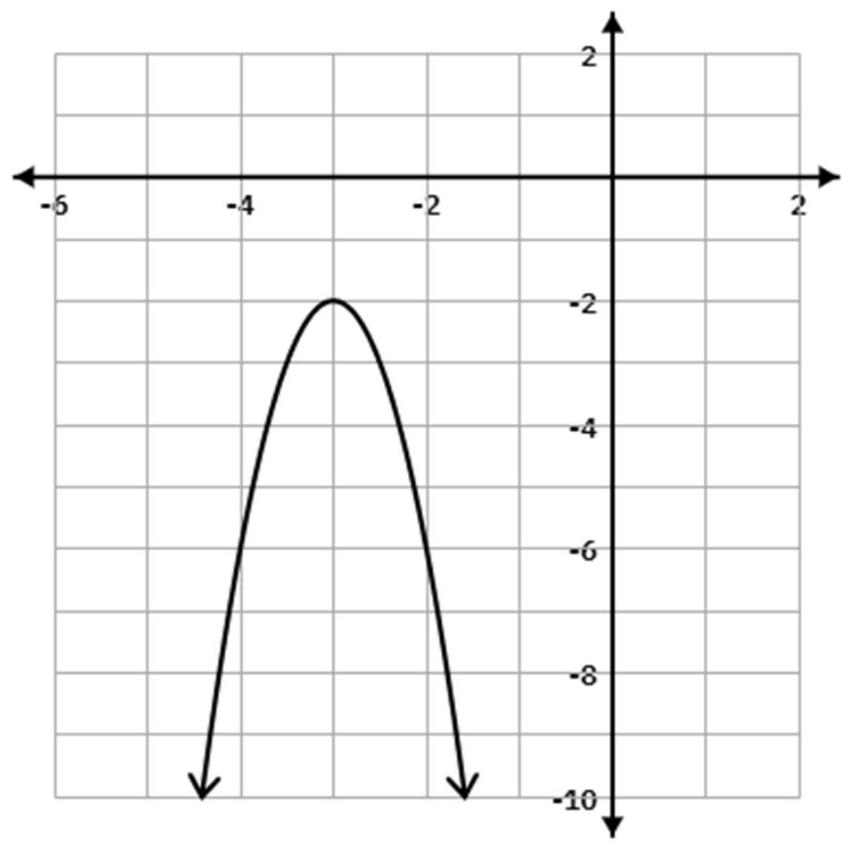
\includegraphics[max width=\textwidth, alt={}, center]{b1ad2e81-5a39-4bac-8cfd-6ebfc7f4a6f6-12_850_854_227_635}\\
13. Write $f(x)$ in vertex form. (2 points)\\
14. Write $f(x)$ in factored form. (1 point)\\
15. Write $f(x)$ in standard form. (1 point)


\end{document}